%\textbf{IBM to write the first version}

%Need 1-2 Pages on Data Fabrication and data masking
%Screen shots of tools?

IBM’s Data Fabrication Platform (DFP) is a web based central platform for generating high-quality data for testing, development, and training. The platform provides a consistent and organisational wide methodology for creating test data. The methodology used is termed “rule guided fabrication”.
The primary DFP use case for fabricating synthetic data contains two actors: a user (initiator) and Database/File (participant). This use case includes two sub-use cases: data modelling and data generation. The data modelling use case includes three sub-use cases: resources and structure definitions, constraint rules definitions and fabrication configuration definitions. The data structure for databases (schema, tables, columns, etc.) is automatically imported, however structural hierarchy of data elements (structs, arrays, tables, fields, types) need to be manually defined by the user. The constraint rules are required to construct a model of the data and thus enable creation of meaningful realistic data vales. Input and output resources are standard relational databases (e.g., DB2, Oracle, PostgreSQL, SQLite), standard file formats (e.g., Flat file, XLS, CSV, XML, JSON) and streaming via MQTT protocol.

In rule guided fabrication, the database logic is extracted automatically and is augmented by application logic and testing logic modelled by the user.
The application logic and the testing logic can be modelled using rules that the platform provides. The platform is also extendable and new rule types can be added by users and automatically integrated into the platform in an organisation-wide manner.
Once the user requests the generation of a certain amount of data into a set of test databases, the platform internally ensures that the generated data satisfies the modelled rules as well as the internal databases consistency requirements.
The platform can generate data from scratch, inflate existing databases, move existing data, and transform data from previously existing resources, such as old test databases or even production data. The platform provides a comprehensive and hybrid solution that can create a mixture of synthetic and real data according to user requirements.

\begin{figure}
    \centering
    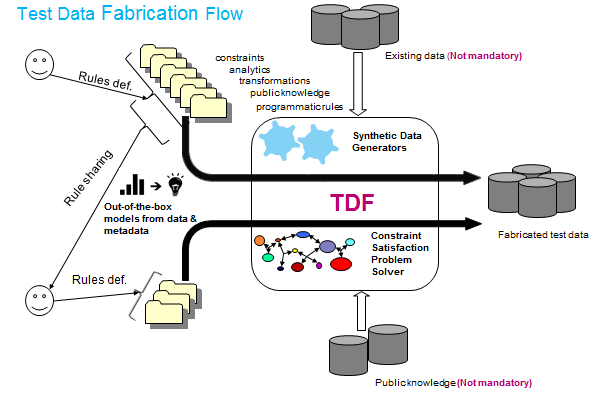
\includegraphics[width=0.45\textwidth]{images/DFPPlatformFlow.png}
    \caption{Flow of Generating Fabricated Data}
    \label{fig:dataFab}
\end{figure}

To overcome the shortcomings of existing data generation techniques, DFP generates data using a proprietary Constraint Satisfaction Problem (CPS) solver (See Figure~\ref{fig:dataFab}). This methodology is generic and flexible for various types of use cases yet also very safe, as all user constraints must be satisfied. The solution does not require access to real or masked data, or to historic actual queries, which all might involve some violation of privacy regulations. Data generation can be constrained directly by the users. These constraints can direct the generation towards desired testing objectives or to realistic database statistics and query behaviour. The platform uses the database schema or the file hierarchical structure, the user requirements via variables and constraints and a fabrication configuration specifying which rules to use and where to write the generated data into. The constraint-problem is solved, and the solution is used to construct the records needed to populate the database or file. A user defines a data project which contains the structure of the data, the constraint rules and the fabrication configuration. In order to construct a constraint satisfaction problem for the solver, the platform analyses the table meta-data and gets table columns’ data type and other properties, e.g., referential integrity constraints. The platform selects a sub-set of the relevant rules and tables using the fabrication configuration. In addition, relevant parent tables may be added due to referential integrity dependencies. Additional default rules are sometimes required as well (PK, Unique Column, string and binary column widths, etc.).
This information is used for the construction of a database table dependency graph. For each table in that graph, starting at root nodes, structural record dependencies are built recursively.

Once the above graphs are built, the fabrication pattern is computed where each target table record is assigned to one of the following fabrication modes: ‘New’, ‘Reuse’ or ‘Other’.
Given the patterns, the graph and the rules, a CSP problem can be created. The CSP has a language used to model a real-world problem. A problem consists of variables and rules. The solution is an assignment of one value for each variable where all the rules are satisfied. The solver finds a random solution. Each time it solves a problem, a new solution is produced. The user does not specify how to solve the problem, but rather focuses on what to solve using the specified rules for a legal solution.
Each table is translated into a CSP variable struct or a CSP vector of variable structs, according to the record type, each table column is translated into a CSP variable. Each of the rules is added to the problem as a CSP constraint.

Finally, the problem is submitted to the solver. The solution is recursively parsed starting the iteration root following the topology of (vectored) record variables. In the case of database project, an SQL insert statement for all table records is created and that SQL insert statement is submitted to the DB for execution. If streaming option is enabled and properly configured, the solution is converted to the relevant format and sent to the messaging broker specified in the configuration. In the case of file projects, the solver result is converted into the relevant file format.



